%%
%% This is file 'hhuthesis-example.tex'
%%
%% Copyright(C) 2020-2021, Wenhan Cao.
%% College of Water Conservancy and Hydropower Engineering, Hohai University.
%%
%% Home Page of the Project:
%% http://github.com/caowenhan/hhuthesis
%%
%% Version:v2.0.0
%% Last update: April 7th,2021.
%% It may be distribute and / or modified under the conditions of the LaTeX Project
%% Public License, either version 1.3c of this license or (at your option) any
%% later version. The latest version of this license is in
%% 
%% http://www.latex-project.org/lppl.txt
%%
%% and version 1.3c or later is part of all distributions of LaTeX version
%% 2008/05/04 or later.
%%

%% 默认博士论文模板 doctor

\documentclass[bachelor]{hhuthesis}

%% 模板选项:本科毕业论文bachelor;学术型硕士论文academicmaster;专业学位硕士论文professionalmaster;非全日制专业学位论文nonfulltimemaster;博士论文doctor

%% 更改数学字体设置,Latin Modern Math 默认的有点细,可选用下列宏包
% \usepackage[bold-style=ISO]{unicode-math}

\begin{document}

%%
%% 封面
%%

%% 国家图书馆封面和中文信息封面
\studentnumber{1209800072}
\classification{TV14}
\securitylevel{无}
\studentgrade{2017级}
\udc{627}
\title{河网地区水力水质特性的\\组合单元解法及反问题的研究}
\vtitle{河网地区水力水质特性的组合单元解法及反问题的研究}
\author{韩中国}

% 专业型硕士\tutorinfoa填写学校指导老师信息,\tutorinfob填写基地指导老师信息
% 其余用户\tutorinfoa填写指导老师姓名&职称,\tutorinfob填写指导老师单位&地址
\tutorinfoa{张长江}
\tutorinfob{河海大学水利水电学院}

\degree{工学博士}
\major{水力学及河流动力学}
\submitdate{2016年7月6日}
\defenddate{2016年9月30日}
\awarded{河~海~大~学\hspace{3em}2016年12月30日}
\chairman{王继承}
%%博士答辩专家为7人,硕士答辩专家为5人,\reviewerf{}和\reviewerg{}可以省略不填。
\reviewera{王继承}
\reviewerb{李生柱}
\reviewerc{徐鹏飞}
\reviewerd{陈\hspace{1em}诚}
\reviewere{吴树人}
\reviewerf{姜大文}
\reviewerg{蒋小为}
\nlcdate{2016年12月}
\nlclocate{中~~国~~$\cdot$~~南~~京}
\institute{河海大学}
\zhtitle{河网地区水力水质特性的组合单元解法及反问题的研究}
\zhsubtitle{无}
\entitle{\hfill Combined Cells Model of Hydraulics and Water Quality of \\River Networks and Its Reverse Problem}
\ensubtitle{None}
\thesislang{汉语}
\abstractlang{汉、英}
\thesispages{198}
\numofwords{11}
\thesiskeywords{河网、力特征、水质特性、污染面、联合解法}
\researchfield{工程水力学及环境水力学}

%% 博士、学术型硕士填写,专业型硕士不用填写
\tutor{张长江~教授}	
\tutorinstitute{河海大学水利水电学院}

%% 专业型硕士填写,其余不用填写
\tutora{}
\tutorainstitute{}
\tutorb{}
\tutorbinstitute{}

%% 英文信息封面
\englishtitle{Combined Cells Model of Hydraulics and Water Quality of River Networks and Its Reverse Problem}
\englishauthor{Han Zhongguo}
\entutor{Professor~~Zhang Changjiang}
\eninstitute{Hohai University}
\englishdepartment{College of Water Conservancy and Hydropower Engineering}
\englishdate{September, 2016}
\enlocate{Nanjing,  P.R.China}
\englishdegree{Doctor of Engineering}

%% 制作国家图书馆封面
\makenlctitle

%% 制作书脊
%\makeverticaltitle

%% 制作中文信息封面
%\makeinfo

%% 制作英文信息封面
\makeeninfo

%% 论文原创性声明和使用授权
\makedeclare

%%
%% 前置部分
%%
\frontmatter

%% 前言,硕士论文不需要可删除
% %%
%% This is file 'preface.tex'
%% It is included by hhuthesis-example.tex for hhuthesis.
%%
%% Copyright(C) 2020, Wenhan Cao
%% College of Water Conservancy and Hydropower Engineering, Hohai University.
%%
%% Version:v1.0.0
%% Last update: July 19th, 2020.
%%
%% Home Page of the Project: https://github.com/caowenhan/thesis
%%
%% This file may be distributed and / or modified under the conditions of the
%% LaTeX Project Public License, either version 1.3c of this license or (at your
%% option) any later version. The latest version of this license is in:
%%
%% http://www.latex-project.org/lppl.txt
%%
%% and version 1.3c or later is part of all distributions of LaTeX version
%% 2008/05/04 or later.
%%
\begin{preface}
我国修建了大量的混凝土坝工程,这些水利工程在防洪、灌溉和发电、通航等方面发挥了巨大的作用。然而,由于我国具有独特的水资源分布特征,有相当一部分混凝土坝修建于高海拔或高纬度的东北、西北等寒冷地区,这些地区普遍存在昼夜温差大、冰冻周期长和年际冻融次数多等特点,容易引发混凝土坝出现冻融与溶蚀等典型渗水病害,导致大坝服役性能衰退,给工程安全造成威胁。因此,科学地分析寒冷地区混凝土坝在渗水病害影响下工作性态演化机制,并对其服役性态进行客观评估,已成为研究的热点。\par
针对上述问题,综合运用数学方法、力学理论、坝工知识和计算机技术,从微观、细观、宏观和整体性态变化及安全角度,系统开展了寒冷地区渗水病害影响下混凝土坝服役性态多尺度分析方法研究,取得以下主要创新性成果:	
\begin{enumerate}
	\item[(1)] 针对坝体混凝土材料多尺度多物相复合属性特征,引入三维微观水化模型,研究了坝体混凝土微观结构特性;采用静水压力与结晶压力复合作用模型,分析了坝体混凝土微观冻融力学性能演化规律;提出水泥基材料析钙溶蚀模型,并采用随机溶蚀算法,探究了坝体混凝土微观溶蚀力学性能演化特性。
	\item[(2)] 分析了砂浆及混凝土材料多尺度物相特征,构建了坝体混凝土材料力学多尺度递进分析表征模型;通过引入数学渐进均匀化理论,以连续损伤力学为支撑,基于多尺度能量积分方法,提出了坝体混凝土材料在冻融和溶蚀两种典型渗水病害影响下力学性能多尺度递进分析模型。	
\end{enumerate}
	
\end{preface}

%% 摘要
%% This is file 'abstract.tex'
%% It is included by hhuthesis-example.tex for hhuthesis.
%%
%% Copyright(C) 2020-2021, Wenhan Cao
%% College of Water Conservancy and Hydropower Engineering, Hohai University.
%%
%% Version:v2.0.0
%% Last update: April 7th, 2021.
%%
%% Home Page of the Project: https://github.com/caowenhan/thesis
%%
%% This file may be distributed and / or modified under the conditions of the
%% LaTeX Project Public License, either version 1.3c of this license or (at your
%% option) any later version. The latest version of this license is in:
%%
%% http://www.latex-project.org/lppl.txt
%%
%% and version 1.3c or later is part of all distributions of LaTeX version
%% 2008/05/04 or later.
%%

\begin{abstract}
	本文首次提出并建立了诸如组合单元水力计算正问题、组合单元水质正问题、水量模型参数反问题、水质边界条件及污染源项反问题等系列成果。主要研究内容如下:
\begin{enumerate}
	\item[(1)] 组合单元水力计算正问题。
	\item[(2)] 组合单元水质正问题。
\end{enumerate}


\keywords{河网;力特征;水质特性;污染面;联合解法}
\end{abstract}

\begin{enabstract}
	This paper makes more systematic and deeper studies on numerical simulations of hydraulics and water quality features of river networks. As a result, a series of achievements such as combined cells model of hydraulics, combined cells model of water quality, roughness parameter reverse problem, waste load reverse problem and simulation of hydraulics boundary condition have been put forward for the first time. The details are as follows:

\begin{enumerate}
\item[(1)] combined cells model of hydraulics.
\item[(2)] combined cells model of water quality.
\end{enumerate}  
 
\enkeywords{River network; Force characteristics; Water quality characteristics; Pollution surface; Joint solution}

\end{enabstract}


%% 符号对照表,可选,如不用可注释掉
% %% This is file 'denotation.tex'
%% It is included by hhuthesis-example.tex for hhuthesis.
%%
%% Copyright(C) 2020, Wenhan Cao
%% College of Water Conservancy and Hydropower Engineering, Hohai University.
%%
%% Version:v1.0.0
%% Last update: July 19th, 2020.
%%
%% Home Page of the Project: https://github.com/caowenhan/thesis
%%
%% This file may be distributed and / or modified under the conditions of the
%% LaTeX Project Public License, either version 1.3c of this license or (at your
%% option) any later version. The latest version of this license is in:
%%
%% http://www.latex-project.org/lppl.txt
%%
%% and version 1.3c or later is part of all distributions of LaTeX version
%% 2008/05/04 or later.
%%

\begin{denotation}
	
\item[\LaTeX] 一个很棒的排版系统
\item[\LaTeXe] 一个很棒的排版系统的最新稳定版
\item[\XeTeX] \LaTeX{}的好兄弟,事实上他有很多个兄弟,但是这个兄弟对各种语言的支持能力都很强
\item[ctex] 成套的中文\LaTeX{}解决方案
\item[\ce{CaCO3}] 碳酸钙
\item[$ e^{\pi{}i}+1=0$] 集自然界五大常数一体的最美方程,欧拉公式

\end{denotation}


%% 加入目录
\tableofcontents

%% 加入图、表索引(同时取消图表索引中章之间的垂直间隔,不需要可以注释)
\let\origaddvspace\addvspace
\renewcommand{\addvspace}[1]{}
%\listoffigures
%\listoftables
\renewcommand{\addvspace}[1]{\origaddvspace{#1}}

%%
%% 正文部分
%%
\mainmatter

%% 各章正文内容
%% This is file 'chapter1.tex'
%% It is included by hhuthesis-example.tex for hhuthesis.
%%
%% Copyright(C) 2020, Wenhan Cao
%% College of Water Conservancy and Hydropower Engineering, Hohai University.
%%
%% Version:v1.0.0
%% Last update: July 19th, 2020.
%%
%% Home Page of the Project: https://github.com/caowenhan/thesis
%%
%% This file may be distributed and / or modified under the conditions of the
%% LaTeX Project Public License, either version 1.3c of this license or (at your
%% option) any later version. The latest version of this license is in:
%%
%% http://www.latex-project.org/lppl.txt
%%
%% and version 1.3c or later is part of all distributions of LaTeX version
%% 2008/05/04 or later.
%%
\chapter{样本章}
\label{chap:sample}
\section{研究的目的和意义}
\label{sec:aim}

水库大坝不仅是调控水资源时空分布、优化水资源配置的重要工程措施,也是江河防洪工程体系的重要组成部分,是经济社会发展不可替代的基础支撑\cite{胡四一2008确保水库大坝安全意义重大任务艰巨}。我国是举世闻名的治水大国,建坝数量、建设规模与技术难度均居世界前列,其中,混凝土坝由于其可靠性高和环境适应能力强等特点,是目前我国大、中型水利工程的主要坝型。然而,由于我国特殊的水电资源分布特征,有相当一部分混凝土坝修建于我国高海拔或高纬度的东北、西北等气候寒冷区域,由于寒冷地区普遍存在昼夜温差大、年平均冰冻周期长和年际冻融次数多等特点,极易导致坝体混凝土材料在严寒气候条件和复杂荷载工况作用下,出现冻融破坏和溶蚀损伤等典型渗水病害问题,进而导致大坝服役性能的衰退,威胁工程服役安全。\par
寒冷地区在地理学领域是指由于高海拔或者高纬度而形成的特别寒冷的气候区域,广义上中国的寒冷地区主要包括整个青藏高原,以及甘肃、内蒙古和新疆的高山地区以及东北和华北部分地区。寒冷地区气候条件十分恶劣,四季气温周期交替变化,气温年变幅大,冰冻期长,导致这些地区水利工程每年需要承受多次冻融循环(我国现场环境年均冻融循环次数分布如图\ref{fig:map}\cite{武海荣2012混凝土冻融环境区划与抗冻性寿命预测}。

\begin{figure}[H]
	\centering
	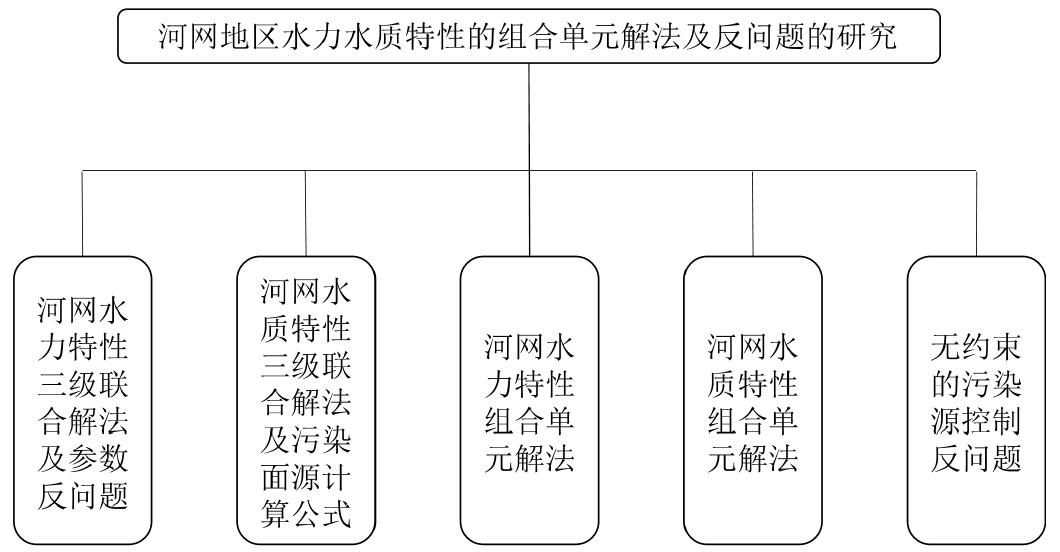
\includegraphics[width=0.75\textwidth]{figure1.jpg}
	\bicaption{我国现场环境年均冻融循环次数分布图}{The average field environmental freezing and thawing times in China}\label{fig:map}
\end{figure}
\section{坝体混凝土材料微观结构特性表征}
本节在对水泥基材料微观尺度基本水化反应和结构特性研究的基础上,引入三维微观水化模型,系统研究坝体混凝土材料三维微观结构特性,从而为后续研究寒冷地区渗水病害影响下坝体混凝土微观力学性能演化特性奠定基础条件。

\subsection{水泥基材料基本水化反应}
硅酸盐水泥生料主要由钙、硅、氧三种化学元素组成的氧化物构成,相应化学成分和简称分别为:\ce{CaO}(C)、\ce{SiO2}(S)、\ce{Al2O3}(A)、\ce{Fe2O3}(F)、\ce{MgO}(M)、\ce{SO3}($\bar{S}$)和\ce{H2O}(H),相应水泥熟料扫描电子显微镜图如图\ref{fig:diagram}。

\begin{figure}[H]
	\centering
	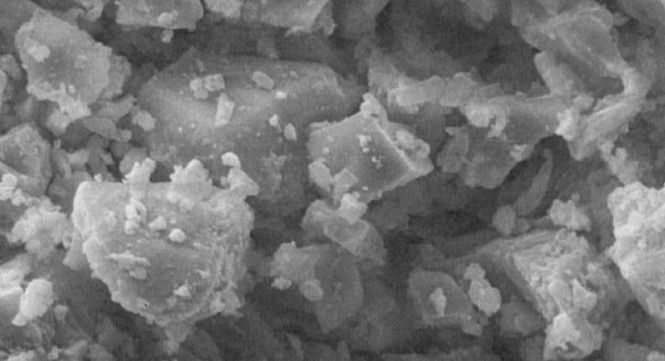
\includegraphics[width=0.75\textwidth]{figure2.jpg}
	\bicaption{硅酸盐水泥熟料颗粒扫描电子显微镜图}{The electron microscope scanning diagram of Portland cement Particle}\label{fig:diagram}
\end{figure}
\subsection{水泥微观水化模型基本原理}
本文主要通过引入HYMOSTRUC 3D模型用于模拟水泥水化反应和水泥基材料微观结构生成。该模型最早由荷兰Technische Universiteit Delft的Klaas van Breugel教授于1991年提出\cite{Delft1991Simulation,钱智炜2010水泥净浆微观结构断裂破坏过程的三维模拟},后经该大学的微观实验室(Microlab)研究人员的开发和完善,逐步形成了比较成熟的水泥微观水化数值计算平台。HYMOSTRUC 3D模型可以综合考虑水泥化学组成、水泥颗粒尺寸分布、矿物掺合料的种类以及水灰比、养护条件等技术参数对水泥水化过程的影响,是迄今为止连续水化模型中较为系统和全面的水泥水化模型,下面重点研究该模型基本特点及其建模原理。
\subsubsection{HYMOSTRUC 3D~基本水化单元}
元胞是HYMOSTRUC~3D模型基本水化单元,元胞边长$S_{x}$及元胞内部水泥颗粒分布主要由水灰比及水泥颗粒PSD决定。基于Rosin-Rammler方程,硅酸盐水泥颗粒PSD可以表示为:
\begin{equation}
	G(x)=1-e^{-bx^{n}}
\end{equation}
\noindent 式中,$x$(μm) 为水泥颗粒尺寸;$b$及$n$为待拟合常数。

\subsection{算例分析}
基于HYMOSTRUC 3D水化模型,采用波兰特水泥CEM~I~42.5~N熟料进行水泥微观水化过程数值模拟,相应水泥熟料化学成分及矿物组成如表\ref{tab:composition}和表\ref{tab:mineral},水泥Blaine值为$380m2/kg$。

\begin{table}[H]\small
	\centering
	\bicaption{波兰特水泥氧化物化学组成成分表}{Chemical composition table of Poland special cement} \label{tab:composition}
	\begin{tabular*}{\textwidth}{@{\extracolsep{\fill}}cccccccccccc}
		\toprule
		氧化物	& \ce{CaO} & \ce{SiO2} & \ce{Al2O3} & \ce{Fe2O3} & \ce{K2O} & \ce{Na2O} & \ce{SO3} & \ce{MgO} & \ce{TiO2} & \ce{Mn3O4} & \ce{P2O5} \\
		\midrule
		百分比(\%) &64.4	&20.36 & 4.96 &
		3.17 &0.64	&0.14	&2.57 &
		2.09	&0.35	&0.14	&0.18 \\
		\bottomrule
	\end{tabular*}
\end{table}

\begin{table}[H]\small
	\centering
	\bicaption{波兰特水泥矿物组成成分表}{Mineral composition of Poland special cement} \label{tab:mineral}
	\begin{tabular*}{\textwidth}{@{\extracolsep{\fill}}ccccc}
		\toprule
		矿物成分	& \ce{C3S} & \ce{C2S} & \ce{C3A} & \ce{C4AF} \\
		\midrule
		百分比(\%) &65.83	&14.76 &7.64 &9.15  \\
		\bottomrule
	\end{tabular*}
\end{table}


%% This is file 'chapter2.tex'
%% It is included by hhuthesis-example.tex for hhuthesis.
%%
%% Copyright(C) 2020-2021, Wenhan Cao
%% College of Water Conservancy and Hydropower Engineering, Hohai University.
%%
%% Version:v2.0.0
%% Last update: April 7th, 2021.
%%
%% Home Page of the Project: https://github.com/caowenhan/thesis
%%
%% This file may be distributed and / or modified under the conditions of the
%% LaTeX Project Public License, either version 1.3c of this license or (at your
%% option) any later version. The latest version of this license is in:
%%
%% http://www.latex-project.org/lppl.txt
%%
%% and version 1.3c or later is part of all distributions of LaTeX version
%% 2008/05/04 or later.
%%
\chapter{河网水力特性三级联合解法及参数反问题}
\label{chap:inverseproblem}
\section{概述}
河网的非恒定流计算通常采用三级联合解法,此方法可归结为一维圣维南方程组的求解问题,即对组成河网的每条河道采用有限差分的隐式格式离散圣维南方程组,得到线性差分方程组。……\par
……
\section{河道控制方程}
描述明渠一维非恒定流的基本方程为一维Saint-Venant 方程组:
\begin{equation}
	\frac{\partial Q}{\partial x}+B_{W}\frac{\partial Z}{\partial t}=q
\end{equation}
\begin{equation}
	\frac{\partial Q}{\partial t}+2u\frac{\partial Q}{\partial x}+(gA-Bu^{2})\frac{\partial Z}{\partial x}-u^{2}\frac{\partial A}{\partial x}+g\frac{n^{2} |u|Q}{R^{4/3}}=0
\end{equation}
\noindent 式中,$t$为时间坐标;$x$为空间坐标;……\par
……\par
……

\section{边界条件}
……\par
……

\section{方程的求解}
……\par
……

\section{参数反问题}
……\par
……

\section{算例分析}
为了验证上述计算方法的可靠性,通常借用正问题的解来构造反问题。即先进行正问题计算,用其结果验证反问题的解。\par
……\par
……\par
计算结果见表\ref{tab:parameter}。

\begin{table}[H]\small	%\small用于控制表格内字体大小为5号字
	\centering
	\bicaption{参数理论值与最优解}{Theoretiacal value and optimal solution of the parameter} \label{tab:parameter}
	\begin{tabular*}{0.75\textwidth}{@{\extracolsep{\fill}}cccc}
		\toprule
		\multicolumn{1}{l}{} & b1     & b2     & b3     \\\midrule
		理论解                  & 22     & 18     & 16     \\
		最优解1                 & 21.986 & 18.048 & 15.997 \\
		最优解2                 & 21.997 & 18.011 & 15.999 \\ \bottomrule
	\end{tabular*}%
\end{table}


……\par
……
\section{本章小结}
本章采用平原河网三级联合解法水量模型模拟河网的水力要素,建立了平原河网
水量模型,对位于长江下游的南通河网进行了模拟运算。\par
……\par
……

% \input{chapters/chapter3}
% \input{chapters/chapter4}
% \input{chapters/chapter5}
% \input{chapters/chapter6}

%% 参考文献样式设定
\bibliographystyle{hhuthesis-numeric}		% 顺序编码式
%% 参考文献,10号字,使用 BibTeX,包含参考文献文件.bib
\bibliography{reference/chap1} %
%\bibliography{reference/chap1}

%%
%% 后置部分
%% 

%% (其后部分无编号)
\backmatter

%% 致谢
%% This is file 'acknowledgement.tex'
%% It is included by hhuthesis-example.tex for hhuthesis.
%%
%% Copyright(C) 2020-2021, Wenhan Cao
%% College of Water Conservancy and Hydropower Engineering, Hohai University.
%%
%% Version:v2.0.0
%% Last update: April 7th, 2021.
%%
%% Home Page of the Project: https://github.com/caowenhan/thesis
%%
%% This file may be distributed and / or modified under the conditions of the
%% LaTeX Project Public License, either version 1.3c of this license or (at your
%% option) any later version. The latest version of this license is in:
%%
%% http://www.latex-project.org/lppl.txt
%%
%% and version 1.3c or later is part of all distributions of LaTeX version
%% 2008/05/04 or later.
%%

\begin{acknowledgement}

本文是在导师张长江教授的精心指导下完成的。值此论文完稿之际,谨向导师及所有帮助过我的各位表示诚挚的谢意。\par
……\par
……\par
还要特别感谢hhuthesis节省了论文排版的时间。
\vspace{5cm}
\begin{flushright}
	作者:韩中国\\
	2016年12月于南京
\end{flushright}

\end{acknowledgement}


%% 附录
% %% This is file 'resume.tex'
%% It is included by hhuthesis-example.tex for hhuthesis.
%%
%% Copyright(C) 2020, Wenhan Cao
%% College of Water Conservancy and Hydropower Engineering, Hohai University.
%%
%% Version:v1.0.0
%% Last update: July 19th, 2020.
%%
%% Home Page of the Project: https://github.com/caowenhan/thesis
%%
%% This file may be distributed and / or modified under the conditions of the
%% LaTeX Project Public License, either version 1.3c of this license or (at your
%% option) any later version. The latest version of this license is in:
%%
%% http://www.latex-project.org/lppl.txt
%%
%% and version 1.3c or later is part of all distributions of LaTeX version
%% 2008/05/04 or later.
%%

\begin{resume}

%% 需要就写,不需要就注释掉	
\resumeitem{个人简历}

本人……。

\researchitem{攻读博士学位期间发表的主要成果} 

\begin{publications}
	\item \textbf{author's name}, Anyone1, Anyone2, et al. Article's title. Journal's title ,2016,2016(12):1-10. (SCI)
	\item \textbf{作者姓名},第二作者等.论文题名[J].期刊名.已录用.(EI)	
\end{publications}

\researchitem{攻读博士学位期间参与的科研项目} 

\begin{projects}
	\item 国家自然科学基金重点项目:基金名称ABCD(编号:XXXXXXXX)
	\item 国家自然科学基金面上项目:基金名称abcd(编号:YYYYYYYY)
\end{projects}

\researchitem{攻读博士学位期间所获的荣誉与奖励} 

\begin{honours}
	\item 2013.06\hspace{1em}获“优秀研究生”荣誉称号
	\item 2016.12\hspace{1em}获河海大学博士研究生国家奖学金
\end{honours}

\end{resume}


\end{document}